%
% wave.tex -- domain for the wave equation
%
% (c) 2019 Prof Dr Andreas Müller, Hochschule Rapperswil
%
\documentclass[tikz,12pt]{standalone}
\usepackage{amsmath}
\usepackage{times}
\usepackage{txfonts}
\usepackage{pgfplots}
\usepackage{csvsimple}
\usetikzlibrary{arrows,intersections,math}
\begin{document}
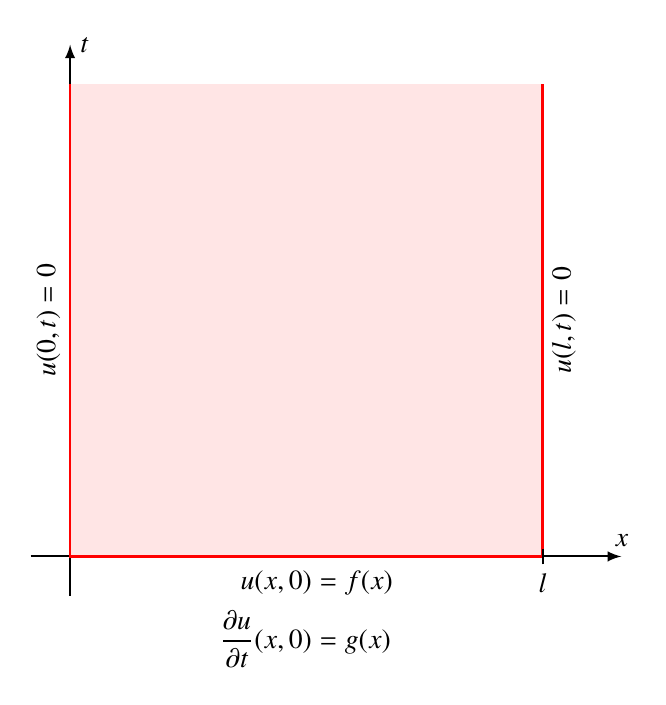
\begin{tikzpicture}[>=latex]

\fill[color=red!10] (0,0) rectangle (6,6);

\draw[->,line width=0.7pt] (-0.5,0)--(7,0) coordinate[label={$x$}];
\draw[->,line width=0.7pt] (0,-0.5)--(0,6.5) coordinate[label={right:$t$}];

\draw[line width=1pt,color=red] (0,6)--(0,0)--(6,0)--(6,6);

\draw[line width=0.7pt] (6,-0.1)--(6,0.1);
\node at (6,-0.1) [below] {$l$};

\node at (3,0) [below] {$
\begin{aligned}
u(x,0)&=f(x)\\
\frac{\partial u}{\partial t}(x,0)&=g(x)
\end{aligned}$};

\node at (6,3) [below,rotate=90] {$u(l,t)=0$};
\node at (0,3) [above,rotate=90] {$u(0,t)=0$};

\end{tikzpicture}
\end{document}

